\documentclass[11pt,a4paper]{article}

\usepackage[left=2.5cm, right=2.5cm]{geometry}
\usepackage[english]{babel}
\usepackage{amsmath,amsfonts,amssymb,amsthm}
\usepackage{amsbsy}
\usepackage{setspace}
\usepackage[shortlabels]{enumitem}

\setstretch{1.1}
\usepackage{float}
\usepackage[dvipsnames]{xcolor}
\usepackage[colorlinks,linkcolor=red,citecolor=green,urlcolor=blue,hypertexnames=true]{hyperref}
\usepackage{graphicx}
\title{}
\author{Ivan Mikhailov}

% Theorem environments
\theoremstyle{plain}
\newtheorem{theorem}{Theorem}[section]
\newtheorem{proposition}[theorem]{Proposition}
\newtheorem{lemma}[theorem]{Lemma}
\newtheorem{claim}[theorem]{Claim}
\newtheorem{corollary}[theorem]{Corollary}

\theoremstyle{definition}
\newtheorem{definition}[theorem]{Definition}
\newtheorem{example}{Example}[section]

\theoremstyle{remark}
\newtheorem{remark}[theorem]{Remark}

\renewcommand{\qedsymbol}{$\spadesuit$}

% Macros
\newcommand{\R}{\mathbb{R}}
\newcommand{\hwdate}{April 6, 2026}
\newcommand{\rthree}{$\R^3$}
\newcommand{\ip}[2]{\langle #1,\, #2 \rangle}

\begin{document}

\thispagestyle{empty}
\begin{flushleft}           
    University of Primorska \\
    FAMNIT
\end{flushleft}

\vspace*{0.2\textheight} 

\begin{center}
    {\LARGE Chapter 2: Lines and Planes in \rthree\  — Summary}\\[1cm]
    {\large Ivan Mikhailov}\\[0.25cm]
    {\large Mathematical Practicum \uppercase\expandafter{\romannumeral 1}}
\end{center}

\vfill

% \maketitle                       % renders title, author, date

\begin{flushleft}
    \hwdate
\end{flushleft}

% ======================= %
\newpage
% ======================= %

\pagenumbering{arabic}
\setcounter{page}{1}

\begin{abstract}
This summary presents the core concepts of lines and planes in \rthree.
Lines are described using a point and a direction vector, while planes are defined by a point and a normal vector, each with multiple equivalent representations.
It covers intersections, distances, and angles between lines, planes, and points, providing key formulas for practical computations.
The summary consolidates essential vector-based techniques for analyzing spatial relationships in three-dimensional space.
The material follows \cite{protter} and \cite{algebra1}.
\end{abstract}

% ======================= %
\newpage
% ======================= %

\tableofcontents
\vspace{1cm}
\listoftables
\vspace{1cm}
\listoffigures

% ======================= %
\newpage
% ======================= %

\section{Lines in \texorpdfstring{\rthree}{R\textasciicircum 3}}
A line in space is determined by a \textbf{point} $P_0(x_0, y_0, z_0)$
and a \textbf{direction vector} $v = (v_1, v_2, v_3)$, as illustrated in Figure~\ref{fig:line}.

\begin{figure}[H]
\centering
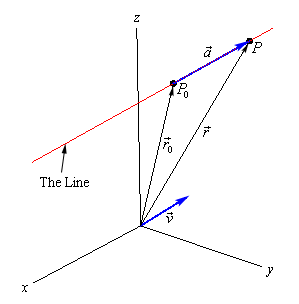
\includegraphics[width=0.6\textwidth]{line.png}
\caption{A line in \rthree\ determined by a point $P_0$ and a direction vector $v$.}
\label{fig:line}
\end{figure}

\subsection{Three equivalent forms}
\subsubsection{Vector form}
\[
r_1 = r_0 + \lambda v, \quad \lambda \in \R
\]

\subsubsection{Parametric form}

\[
\begin{cases}
x = x_0 + \lambda v_1 \\
y = y_0 + \lambda v_2 \\
z = z_0 + \lambda v_3
\end{cases}
\]

\subsubsection{Canonical form}
\[
\frac{x - x_0}{v_1} = \frac{y - y_0}{v_2} = \frac{z - z_0}{v_3} = \lambda
\]
Requires all $v_i \neq 0$.\renewcommand{\thefootnote}{\dag}\footnote{If a component $v_i = 0$, the corresponding fraction is omitted and replaced by the condition $x_i = x_{i,0}$ instead. For example, if $v_3 = 0$, the canonical form becomes $\frac{x-x_0}{v_1} = \frac{y-y_0}{v_2}$ together with $z = z_0$.}\renewcommand{\thefootnote}{\arabic{footnote}}

\vspace{\baselineskip}

The representation is not unique — \textit{any} point on the line can serve as the base point, and any nonzero scalar multiple of $v$ gives the same line.

% ======================= %
\newpage
% ======================= %

\section{Planes in \texorpdfstring{\rthree}{R\textasciicircum 3}}
A plane is determined by a \textbf{point} $R_0(x_0, y_0, z_0)$ and a \textbf{normal vector} $n = (a, b, c)$ perpendicular to the plane.
$\langle u, v \rangle = \sum_{i=1}^{3} u_i v_i$ denotes the dot product of vectors $u$ and $v$.

\subsection{Three equivalent forms}

\subsubsection{Vector form}
\[
\langle n, r - r_0 \rangle = 0
\]

\subsubsection{General form}
\[
ax + by + cz = d, \quad \text{where } d = ax_0 + by_0 + cz_0
\]

The general form is obtained from the vector form by expanding the dot product:
\begin{align*}
\langle n,\, r - r_0 \rangle &= 0 \\
a(x - x_0) + b(y - y_0) + c(z - z_0) &= 0 \\
ax - ax_0 + by - by_0 + cz - cz_0 &= 0 \\
ax + by + cz &= ax_0 + by_0 + cz_0 \\
             &= d.
\end{align*}

\subsubsection{Vector parametric description}
\[
r_0 + \lambda u + \mu v, \quad \lambda, \mu \in \R
\]
where $u, v$ are two linearly independent vectors lying in the plane.

\vspace{\baselineskip}

To convert parametric $\rightarrow$ general: find 
$n = u \times v$ (the cross product of the two direction vectors), then substitute the support point to get $d$.

\vspace{\baselineskip}

Three noncollinear points $A, B, C$ also determine a plane via:
\[
\begin{vmatrix}
x - x_0 & y - y_0 & z - z_0 \\
x_1 - x_0 & y_1 - y_0 & z_1 - z_0 \\
x_2 - x_0 & y_2 - y_0 & z_2 - z_0
\end{vmatrix} = 0
\]

% ======================= %
\newpage
% ======================= %

\section{Intersections}

\subsection{Two lines}

Two lines in \rthree\ fall into one of the following configurations:
\begin{enumerate}[label=\roman*.]
    \item \textbf{Intersecting} — exactly one point in common;
    \item \textbf{Parallel} — direction vectors are proportional, no intersection;
    \item \textbf{Identical} — infinitely many points in common (same line);
    \item \textbf{Skew} — not parallel and do not intersect (only possible in \rthree).
\end{enumerate}

Lines $\ell_1 = r_1 + \lambda_1 v_1$ and
$\ell_2 = r_2 + \lambda_2 v_2$ intersect iff there exist
$\lambda_1, \lambda_2$ such that:
\[
r_1 + \lambda_1 v_1 = r_2 + \lambda_2 v_2
\]
This gives a system of 3 equations; check consistency in all three coordinates.

\subsection{Line and plane}

Substitute the parametric line $\ell = r_0 + \lambda v$ into the plane equation 
$ax + by + cz = d$ and solve for $\lambda$. Then substitute back to get the intersection point.  

\begin{itemize}[label={$\rightarrow$}]
    \item If $\langle n, v \rangle \neq 0$: unique solution exists — the line meets the plane at exactly one point.
    \item If $\langle n, v \rangle = 0$ and the point $r_0$ does not satisfy the plane equation: no solution — the line is parallel to the plane.
    \item If $\langle n, v \rangle = 0$ and $r_0$ lies on the plane: all $\lambda \in \R$ satisfy it — the line lies entirely in the plane.
\end{itemize}

\subsection{Two planes}

Two non-parallel planes intersect in a \textbf{line}. Solve the system of two plane equations, express two unknowns in terms of the third (assign it parameter $\lambda$), and write the result in vector form.

% ======================= %
\newpage
% ======================= %

\section{Distances}

Table~\ref{tab:distances} summarises the main distance formulas covered in this section.

\subsection{Point to line}

Let $R_1$ be the point, $\ell = r_0 + \lambda v$ the line:
\[
\Delta = \frac{|(R_1 - r_0) \times v|}{|v|}
\]

\subsection{Point to plane}

Let $R_1$ be the point, $\Pi$ a plane with normal $n$, and $R_0$ any point on $\Pi$:
\begin{equation}
\Delta = \frac{|\langle R_1 - R_0, n \rangle|}{|n|}
\label{eq:dist-pt-plane}
\end{equation}

\begin{example}
Find the distance from the point $R_1 = (1, 2, 3)$ to the plane $2x + y - z = 4$.

\noindent Taking $n = (2, 1, -1)$ and $R_0 = (2, 0, 0)$ on the plane, Equation~\eqref{eq:dist-pt-plane} gives:
\begin{align*}
\Delta &= \frac{|\ip{R_1 - R_0}{n}|}{|n|} \\
       &= \frac{|\ip{(-1,\, 2,\, 3)}{(2,\, 1,\, -1)}|}{\sqrt{4+1+1}} \\
       &= \frac{|-2 + 2 - 3|}{\sqrt{6}} \\
       &= \frac{3}{\sqrt{6}} \\
       &= \frac{\sqrt{6}}{2}.
\end{align*}
\end{example}

\subsection{Two parallel lines}

Check parallelism: $v_1 \times v_2 = 0$ (equivalently, $v_1$ and $v_2$ are linearly dependent).
Distance = distance from any point on $\ell_1$ to $\ell_2$ (use the point-to-line formula).

\subsection{Two skew lines}

Lines that are not parallel and do not intersect. Formula:
\[
\Delta = \frac{|\langle v_1 \times v_2, r_2 - r_1 \rangle|}{|v_1 \times v_2|}
\]

\subsection{Line and parallel plane}

First verify parallelism: $\langle n, v \rangle = 0$.
Distance = distance from any point on the line to the plane (use Equation~\eqref{eq:dist-pt-plane}).

\subsection{Two parallel planes}

First verify: $n_1 = \alpha n_2$ for some scalar $\alpha$.
Distance = distance from any point on one plane to the other plane.

\begin{table}[H]
\centering
\begin{tabular}{|l || c | c|}
\hline
\textbf{Configuration} & \textbf{Formula} \\
\hline
\hline
Point to line & $\dfrac{|(R_1 - r_0) \times v|}{|v|}$ \\[10pt]
\hline
Point to plane & $\dfrac{|\ip{R_1 - R_0}{n}|}{|n|}$ \\[10pt]
\hline
Two parallel lines & reduce to point-to-line \\[4pt]
\hline
Two skew lines & $\dfrac{|\ip{v_1 \times v_2}{r_2 - r_1}|}{|v_1 \times v_2|}$ \\[10pt]
\hline
Line and parallel plane & reduce to point-to-plane \\[4pt]
\hline
Two parallel planes & reduce to point-to-plane \\[4pt]
\hline
\end{tabular}
\caption{Summary of distance formulas for configurations in \rthree.}
\label{tab:distances}
\end{table}

% ======================= %
\newpage
% ======================= %

\section{Angles}

\subsection{Between two lines}

The angle $\phi$ is always taken as \textbf{acute}:
\[
\cos \phi = \frac{|\ip{v_1}{v_2}|}{|v_1| \cdot |v_2|}
\]

\begin{theorem}[Perpendicularity of lines]
Two lines with direction vectors $v_1$ and $v_2$ are perpendicular if and only if\/ $\ip{v_1}{v_2} = 0$.
\end{theorem}

\begin{proof}
The angle formula gives $\cos\phi = \dfrac{|\ip{v_1}{v_2}|}{|v_1|\cdot|v_2|}$.
Perpendicularity means $\phi = 90^\circ$, so $\cos\phi = 0$, which holds if and only if $\ip{v_1}{v_2} = 0$.
\end{proof}

\subsection{Between a line and a plane}

The angle $\phi$ is between the line and its projection onto the plane:
\[
\sin \phi = \frac{|\langle v, n \rangle|}{|v| \cdot |n|}
\]
where $n$ is the normal to the plane. Equivalently: $\phi = 90^\circ - \beta$, where $\beta$ is the angle between $v$ and $n$.

\subsection{Between two planes}

The angle equals the angle between the normal vectors:
\[
\cos \phi = \frac{|\ip{n_1}{n_2}|}{|n_1| \cdot |n_2|}
\]

\begin{proposition}[Orthogonality of planes]
Two planes with normal vectors $n_1$ and $n_2$ are \textbf{orthogonal} if and only if\/ $\ip{n_1}{n_2} = 0$.
\end{proposition}

\begin{proof}
From the angle formula, $\cos\phi = \dfrac{|\ip{n_1}{n_2}|}{|n_1|\cdot|n_2|}$.
The planes are orthogonal when $\phi = 90^\circ$, i.e.\ $\cos\phi = 0$, which occurs if and only if $\ip{n_1}{n_2} = 0$.
\end{proof}

% ======================= %
\newpage
% ======================= %

\begin{thebibliography}{99}
\sloppy

\bibitem{protter}
P.~M.~Protter and C.~B.~Morrey,
\textit{College Calculus with Analytic Geometry},
2nd~ed., Addison-Wesley, Reading, MA, 1977.

\bibitem{algebra1}
\textit{Algebra I --- Lecture Notes},
University of Primorska FAMNIT\@.
Available at: \url{https://e.famnit.upr.si/pluginfile.php/747259/mod_resource/content/19/Algebra%201%20lecture%20notes_V3.pdf}

\end{thebibliography}

\end{document}